%%%%%%%%%%%%%%%%%%%%%%%%%%%%%%%%%%%%%%%%%%%%%%%%%%%%%%%%%%%%%%%%%%%%%%%%%%%%%%%%%%%%%%%%%%%%%%%%
%
% CS484 Written Question Template
%
% Acknowledgements:
% The original code is written by Prof. James Tompkin (james_tompkin@brown.edu).
% The second version is revised by Prof. Min H. Kim (minhkim@kaist.ac.kr).
%
% This is a LaTeX document. LaTeX is a markup language for producing 
% documents. Your task is to fill out this document, then to compile 
% it into a PDF document. 
%
% 
% TO COMPILE:
% > pdflatex thisfile.tex
%
% If you do not have LaTeX and need a LaTeX distribution:
% - Personal laptops (all common OS): www.latex-project.org/get/
% - We recommend latex compiler miktex (https://miktex.org/) for windows,
%   macTex (http://www.tug.org/mactex/) for macOS users.
%   And TeXstudio(http://www.texstudio.org/) for latex editor.
%   You should install both compiler and editor for editing latex.
%   The another option is Overleaf (https://www.overleaf.com/) which is 
%   an online latex editor.
%
% If you need help with LaTeX, please come to office hours. 
% Or, there is plenty of help online:
% https://en.wikibooks.org/wiki/LaTeX
%
% Good luck!
% Min and the CS484 staff
%
%%%%%%%%%%%%%%%%%%%%%%%%%%%%%%%%%%%%%%%%%%%%%%%%%%%%%%%%%%%%%%%%%%%%%%%%%%%%%%%%%%%%%%%%%%%%%%%%
%
% How to include two graphics on the same line:
% 
% \includegraphics[width=0.49\linewidth]{yourgraphic1.png}
% \includegraphics[width=0.49\linewidth]{yourgraphic2.png}
%
% How to include equations:
%
% \begin{equation}
% y = mx+c
% \end{equation}
% 
%%%%%%%%%%%%%%%%%%%%%%%%%%%%%%%%%%%%%%%%%%%%%%%%%%%%%%%%%%%%%%%%%%%%%%%%%%%%%%%%%%%%%%%%%%%%%%%%

\documentclass[11pt]{article}

\usepackage[english]{babel}
\usepackage[utf8]{inputenc}
\usepackage[colorlinks = true,
            linkcolor = blue,
            urlcolor  = blue]{hyperref}
\usepackage[a4paper,margin=1.5in]{geometry}
\usepackage{stackengine,graphicx}
\usepackage{fancyhdr}
\setlength{\headheight}{15pt}
\usepackage{microtype}
\usepackage{times}

% From https://ctan.org/pkg/matlab-prettifier
\usepackage[numbered,framed]{matlab-prettifier}

\frenchspacing
\setlength{\parindent}{0cm} % Default is 15pt.
\setlength{\parskip}{0.3cm plus1mm minus1mm}

\pagestyle{fancy}
\fancyhf{}
\lhead{Homework 5 Questions}
\rhead{CS484}
\rfoot{\thepage}

\date{}

\title{\vspace{-1.5cm}Homework 5 Questions}


\begin{document}
\maketitle
\vspace{-3cm}
\thispagestyle{fancy}

\section*{Instructions}
\begin{itemize}
  \item 3 questions.
  \item Write code where appropriate.
  \item Feel free to include images or equations.
  \item Please make this document anonymous.
  \item \textbf{Please use only the space provided and keep the page breaks.} Please do not make new pages, nor remove pages. The document is a template to help grading. If you need extra space, please use and refer to new pages at the end of the document.
\end{itemize}

\section*{Questions}

\paragraph{Q1:} Given a linear classifier, how might we handle data that are not linearly separable? How does the \emph{kernel trick} help in these cases? (See course slides in supervised learning, plus your own research.)

%%%%%%%%%%%%%%%%%%%%%%%%%%%%%%%%%%%
\paragraph{A1:} Your answer here.

For non linearly separable data, we can map them to a higher-dimensional space. After they mapped to higher dimensional feature space, the training set is separable linearly. For this mapping, we can use kernel trick. Kernel trick define a kernel function K such that
\begin{equation}
K(x_{i}, x_{j} ) =\phi(x_{i} ) \cdot \phi (x_{j} )
\end{equation}
instead of explicitly computing the lifting transformation (below) for all data.
\begin{equation}
    \phi:X \rightarrow V
\end{equation}
For use this equation, the kernel function must be symmetric and satisfy Mercer's condition. Then the function is semi-definite, and the solution of SVM with the kernel function is global optimum. Then, the kernel function gives a nonlinear decision boundary in the original feature space.
\begin{equation}
    \Sigma\alpha_{i}y_{i}\phi(x_{i})\cdot\phi(x) + b = \Sigma\alpha_{i}y_{i}K(x_{i}, x) + b
\end{equation}
For classification, the kernels such as polynomial kernel, Sigmoid kernel, Radial kernel and Gaussian kernel are used.

%%%%%%%%%%%%%%%%%%%%%%%%%%%%%%%%%%%

\pagebreak
\paragraph{Q2:} In machine learning, what are bias and variance? When we evaluate a classifier, what are overfitting and underfitting, and how do these relate to bias and variance?

%%%%%%%%%%%%%%%%%%%%%%%%%%%%%%%%%%%
\paragraph{A2:} Your answer here.


Bias (accuracy) is the difference between the expected (or average) prediction of our model and the correct value. It occurs due to inaccurate assumptions/simplifications. Variance(precision) is the amount that the estimate of the target function will change if different training data was used.

Underfitting is the situation where the model is too simple to represent all the relevant class characteristics. It may occur because the model has too few parametersm so the model is not flexible. In underfitting, bias is high but variance is low. Also, both training error and test error are high.

Overfitting is the situation where the model is too complex and fits irrelevant characteristics (noise) in the data. It may occur because the model has too many parameters, so the model is too much sensitive to sample. In overfitting, bias is low but variance is high. Also, training error is low but test error is high. 


\begin{figure}[h]
    \centering
    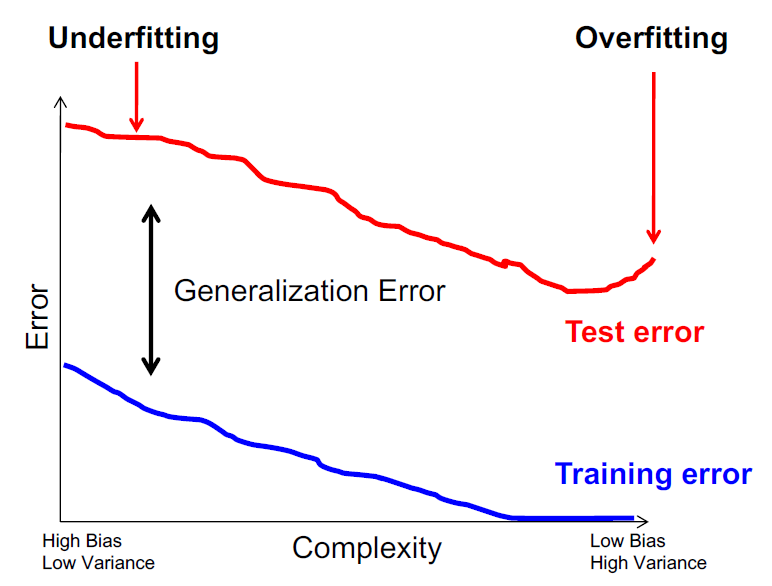
\includegraphics[width=9cm]{questions/A2.PNG}
    \caption{Underfitting and Overfitting with model Complexity}
    \label{fig1}
\end{figure}

%%%%%%%%%%%%%%%%%%%%%%%%%%%%%%%%%%%

% Please leave the pagebreak
\pagebreak
\paragraph{Q3:} The way that the bag of words representation handles the spatial layout of visual information can be both an advantage and a disadvantage. Describe an example scenario for each of these cases, plus describe a modification or additional algorithm which can overcome the disadvantage. 

How might we evaluate whether bag of words is a good model?

%%%%%%%%%%%%%%%%%%%%%%%%%%%%%%%%%%%
\paragraph{A3:} Your answer here.


It has advantages. If there are two cars that have big geometric or within-class variations (but have same features such as wheels, light, etc.), the bag of words can correctly recognize two cars because it only consider histograms while other geometric models can't. 


It has disadvantages. It cannot consider the semantic context, because it only consider the histogram. Suppose that there are two images that are totally different (one has a human face, and one has a mixture of eyes, nose, and lips but not looks like a face.). If they have the same histogram, they will be considered same by bag of words. For overcome this problem, spatial pyramid pooling(SPP) is used. SPP is a collection of orderless representation at several levels of resolution (Figure~\ref{fig2}). Because SPP use all the repeatedly subdivided local sections' histograms for classification, it has more spatial information.


We can measure how much the bag of words is good at producing good classification results. By comparison with other geometric feature such as SIFT while fix the classifier model, if the bag of words is better at classification than others, the method will be a good model.


\begin{figure}[h]
    \centering
    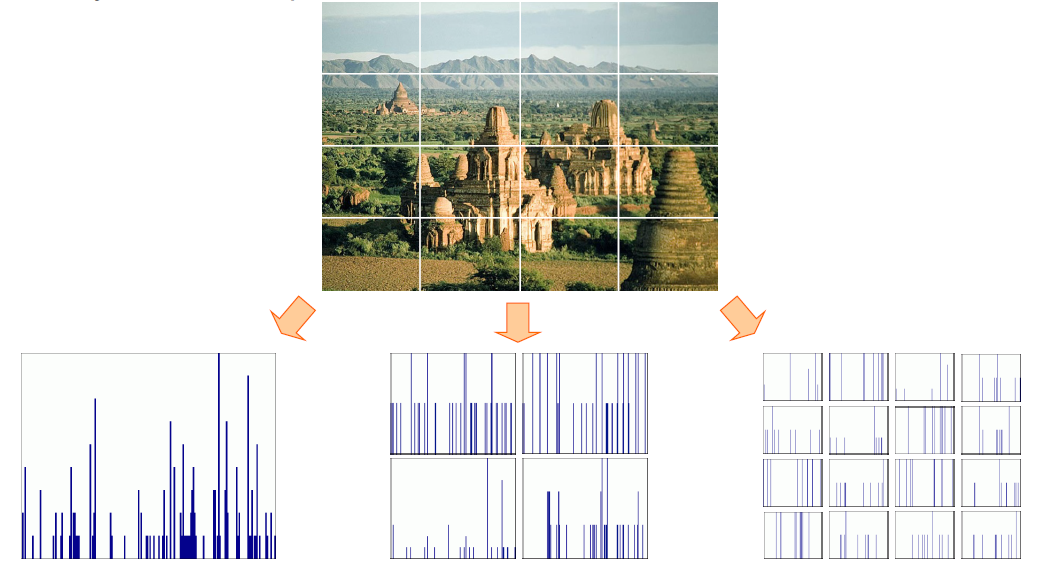
\includegraphics[width=9cm]{questions/SPP.PNG}
    \caption{Spatial Pyramid Pooling (Lazebnik et al.)}
    \label{fig2}
\end{figure}
%%%%%%%%%%%%%%%%%%%%%%%%%%%%%%%%%%%

% If you really need extra space, uncomment here and use extra pages after the last question.
% Please refer here in your original answer. Thanks!
%\pagebreak
%\paragraph{AX.X Continued:} Your answer continued here.



\end{document}
